\chapter*{Appendix}

\section{SeqAcc Operation}
\label{section:appendixseqacc}

\subsection{Charge Redistribution}

take from y2q1 

\subsection{Write and Read}

could be taken from the early Y2Q2 report

\subsection{ADC Design}

take from Y2Q3 report

\subsection{QRAcc Bitcell Design}

can take from the early Y2Q1 report

Lorem Ipsum dolor sit amet, consectetur adipiscing elit. Sed do eiusmod tempor incididunt ut labore et dolore magna aliqua. Ut enim ad minim veniam, quis nostrud exercitation ullamco laboris nisi ut aliquip ex ea commodo consequat. Duis aute irure dolor in reprehenderit in voluptate velit esse cillum dolore eu fugiat nulla pariatur. Excepteur sint occaecat cupidatat non proident, sunt in culpa qui officia deserunt mollit anim id est laborum.

\section{QLinear Operations}
\label{section:appendixqlinearops}
Lorem Ipsum dolor sit amet, consectetur adipiscing elit. Sed do eiusmod tempor incididunt ut labore et dolore magna aliqua. Ut enim ad minim veniam, quis nostrud exercitation ullamco laboris nisi ut aliquip ex ea commodo consequat. Duis aute irure dolor in reprehenderit in voluptate velit esse cillum dolore eu fugiat nulla pariatur. Excepteur sint occaecat cupidatat non proident, sunt in culpa qui officia deserunt mollit anim id est laborum.

\section{QRAcc CSRs and Configuration Registers}
\label{section:appendixqracc_csrs}
\begin{longtable}{@{}llll@{}}
\caption{CSR 0: Main Control Register Bit Fields} \\
\toprule
Bits & Field Name & R/W & Description \\ \midrule
\endfirsthead
\multicolumn{4}{c}%
{{\bfseries \tablename\ \thetable{} -- continued from previous page}} \\
\toprule
Bits & Field Name & R/W & Description \\ \midrule
\endhead
\bottomrule
\endfoot
\endlastfoot
2:0 & \texttt{csr\_main\_trigger} & W & Main trigger for the controller. See Table \ref{tab:triggers}. \\
3 & \texttt{csr\_main\_clear} & W & Clears the controller state. \\
4 & \texttt{csr\_main\_busy} & R & Indicates if the controller is not in the idle state. \\
5 & \texttt{inst\_write\_mode} & W & Set to 1 if writing instructions for a microcode loop. \\
11:8 & \texttt{internal\_state} & R & The internal state of the controller FSM for debugging. \\
12 & \texttt{preserve\_ifmap} & W & If set, the input feature map is preserved after computation. \\
\end{longtable}

\begin{longtable}{@{}llll@{}}
\caption{CSR 1: Layer Configuration Register Bit Fields} \\
\toprule
Bits & Field Name & R/W & Description \\ \midrule
\endfirsthead
\multicolumn{4}{c}%
{{\bfseries \tablename\ \thetable{} -- continued from previous page}} \\
\toprule
Bits & Field Name & R/W & Description \\ \midrule
\endhead
\bottomrule
\endfoot
\endlastfoot
0 & \texttt{binary\_cfg} & W & 1 for binary mode, 0 for bipolar mode. \\
1 & \texttt{unsigned\_acts} & W & 1 for unsigned activations, 0 for signed. \\
7:4 & \texttt{adc\_ref\_range\_shifts} & W & ADC reference range shifts. \\
11:8 & \texttt{filter\_size\_y} & W & Filter dimension in the Y direction. \\
15:12 & \texttt{filter\_size\_x} & W & Filter dimension in the X direction. \\
19:16 & \texttt{stride\_y} & W & Stride in the Y direction. \\
23:20 & \texttt{stride\_x} & W & Stride in the X direction. \\
27:24 & \texttt{n\_input\_bits\_cfg} & W & Number of bits for input data. \\
31:28 & \texttt{n\_output\_bits\_cfg} & W & Number of bits for output data. \\
\end{longtable}

\begin{longtable}{@{}lllll@{}}
\caption{CSR 2 \& 3: Feature Map Dimension Bit Fields} \\
\toprule
Register & Bits & Field Name & R/W & Description \\ \midrule
\endfirsthead
\multicolumn{5}{c}%
{{\bfseries \tablename\ \thetable{} -- continued from previous page}} \\
\toprule
Register & Bits & Field Name & R/W & Description \\ \midrule
\endhead
\bottomrule
\endfoot
\endlastfoot
CSR 2 & 15:0 & \texttt{input\_fmap\_dimx} & W & Input fmap dimension X. \\
CSR 2 & 31:16 & \texttt{input\_fmap\_dimy} & W & Input fmap dimension Y. \\
CSR 3 & 15:0 & \texttt{output\_fmap\_dimx} & W & Output fmap dimension X. \\
CSR 3 & 31:16 & \texttt{output\_fmap\_dimy} & W & Output fmap dimension Y. \\
\end{longtable}

\begin{longtable}{@{}llll@{}}
\caption{CSR 4: Channel Configuration Bit Fields} \\
\toprule
Bits & Field Name & R/W & Description \\ \midrule
\endfirsthead
\multicolumn{4}{c}%
{{\bfseries \tablename\ \thetable{} -- continued from previous page}} \\
\toprule
Bits & Field Name & R/W & Description \\ \midrule
\endhead
\bottomrule
\endfoot
\endlastfoot
15:0 & \texttt{num\_input\_channels} & W & Number of input channels. \\
31:16 & \texttt{num\_output\_channels} & W & Number of output channels. \\
\end{longtable}

\begin{longtable}{@{}llll@{}}
\caption{CSR 5: Mapped Matrix Offset Bit Fields} \\
\toprule
Bits & Field Name & R/W & Description \\ \midrule
\endfirsthead
\multicolumn{4}{c}%
{{\bfseries \tablename\ \thetable{} -- continued from previous page}} \\
\toprule
Bits & Field Name & R/W & Description \\ \midrule
\endhead
\bottomrule
\endfoot
\endlastfoot
15:0 & \texttt{mapped\_matrix\_offset\_x} & W & Mapped matrix offset in X. \\
31:16 & \texttt{mapped\_matrix\_offset\_y} & W & Mapped matrix offset in Y. \\
\end{longtable}

\begin{longtable}{@{}llll@{}}
\caption{CSR 6: Padding Information Bit Fields} \\
\toprule
Bits & Field Name & R/W & Description \\ \midrule
\endfirsthead
\multicolumn{4}{c}%
{{\bfseries \tablename\ \thetable{} -- continued from previous page}} \\
\toprule
Bits & Field Name & R/W & Description \\ \midrule
\endhead
\bottomrule
\endfoot
\endlastfoot
3:0 & \texttt{padding} & W & Set to 1 to enable zero-padding. \\
11:4 & \texttt{padding\_value} & W & Value to use for padding. \\
\end{longtable}



\section{On the possibility of masking writes instead of reducing bins}
\label{section:appendixmasking_writes}

In cases of regular non-bitmasking enabled SRAM, this idea is impossible. However, if the SRAM is bitmasking enabled, it is possible to mask writes to the SRAM. Then, it is possible to only write the useful portions of the matrices onto the SRAM. Combined with QRAcc's column and row masking, this can work as an alternative to MARP while still making use of powerful system-level optimizing single-mapping DNN compilers like CIMLoop, LionHeart, and ZigZag. 

We need QRAcc's row and column masking because with a bitmasking scheme, large matrices left over in the AIMC memory array will not be overwritten by zeros. If the inputs and outputs of those portions are not masked away, (1) unnecessary computational power will be utilized (if the inputs are not maskeed) and (2) the outputs will be incorrect (if the outputs are not masked).

I believe this is actually a pretty good idea for future work. It would allow the use of existing DNN compilers that do not support multi-mapping, while still optimizing for the fewest possible writes.

On the other hand, MARP is also able to solve mappings for multicore AIMC accelerators for whom all the matrices are loaded in all at once. This is not possible with the masking scheme, as the masking scheme essentially evicts the matrices that are not needed for the current inference.

\section{Extra MARP experiments}
\label{section:appendixextra_marp_experiments}

\begin{figure}[htbp]
    \centering
    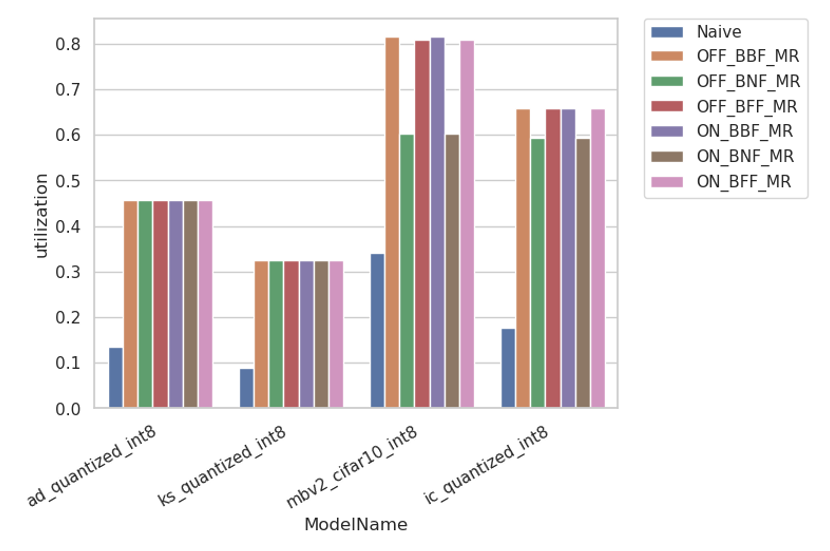
\includegraphics[width=\textwidth]{images/appendix/mlperftiny_utilization_vs_packer.png}
    \caption{Utilization achieved on the MLPerfTiny models for various variants of the MaxRects (MR) algorithm. Different rectpack variants achieve utilizations, but using rectangular packing always improves both compared to single-mapping.}
\end{figure}

\begin{figure}[htbp]
    \centering
    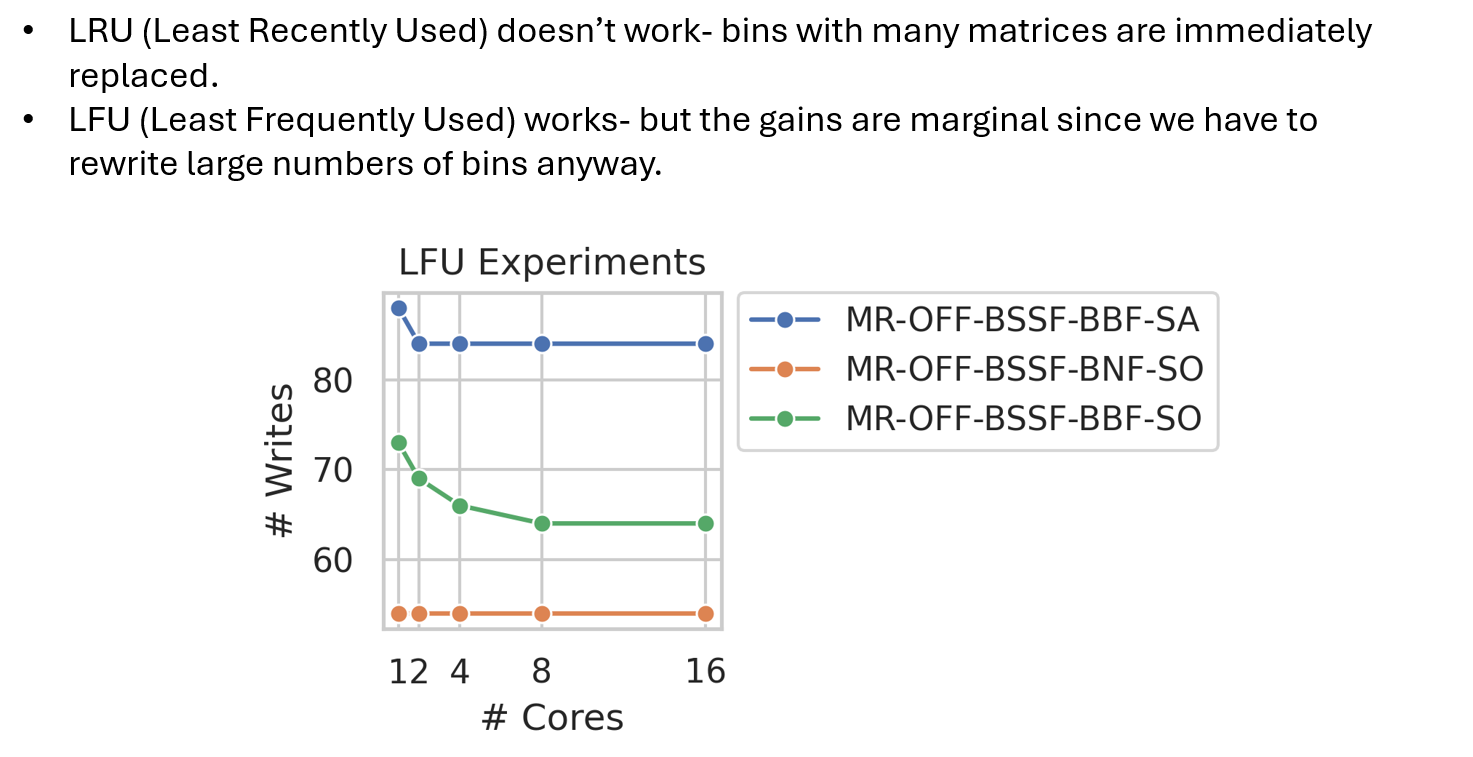
\includegraphics[width=\textwidth]{images/appendix/marp_multicore.png}
    \caption{Multicore experiments with MARP for MobileNetV2}
\end{figure}


\section{SNR Analysis of QRAcc}
\label{section:appendixsnr_analysis}

already in y2q3 report

\subsection{Per-layer SNR on MBV2}

raw data already there, analysis needed.